%`preamble' precedes the main text
\documentclass[12pt, a4paper]{article}

%some important packages
\usepackage[T1]{fontenc}					%package to set font encoding
\usepackage[latin1]{inputenc}				%package to set input encoding
\usepackage[section]{placeins}

%\usepackage[ngerman]{babel} 				%option for paper in german
\usepackage{graphicx} 						%package to include graphics
\usepackage{setspace} 						%package to set space between lines
\usepackage{lscape} 							%package to rotate pages
\usepackage{lipsum} 							%package for random text, delete \lipsum[1]-command when you write your own text
\usepackage{booktabs} 						%package for nice tables
\usepackage{amsmath,amsfonts,amssymb} 	%packages for LaTeX that provides various features to facilitate writing math 									
												%formulas and to improve the typographical quality of their output 
\usepackage{array}							%package for extending array and tabular environments
\usepackage{textcomp}						%package support of the text companion fonts
\usepackage{exscale} 							%package for nice summation sign 
\usepackage{tabularx} 						%package for column width and linebreaks in table cells
\usepackage{natbib}							%package for bibliography
\usepackage{ragged2e} 						%package provides less extreme raggedness than the standard LaTeX commands \flushleft and \flushright
\usepackage{multirow}           					%package to combine cells in tables
\usepackage{eurosym} 						%package to get eurosymbol per \euro
\usepackage{verbatim}						% package for verbatim evironment
\usepackage{float}						%package to define position of tables and figures
\usepackage{color}
%adjustment of page parameters
\usepackage[left=3cm, right=2cm, top=2.5cm, bottom=2.5cm]{geometry}
\renewcommand{\baselinestretch}{1.5} 		%line spacing is set to 1.5
\setlength{\footnotesep}{10.0pt}				%space between footnote and text


%title
\title{{\Large Do voting systems affect segregation\footnote{This paper was written as a term paper in the course XYZ at the Chair of Economics VI: Empirical Economics, Prof. Dr. Mario Larch, University of Bayreuth.}}\\
\vspace{3mm}{\Large Term Paper, Software Engineering for Economists}%options: BA Thesis, MA Thesis etc.
}

%author
\author{Julia Baumann\footnote{4th semester, BA Economics. Student No.: 2323235. Address: Joseph-Schumpeter-Allee 42, 95444 Bayreuth. Tel.: +31 415 926 535 897. Email: market.frictions@uni-bayreuth.de.}\\ Tadas Gedminas\\Axel Purwin}
\date{Autumn 2017}
%beginning of the main text
\begin{document}

\maketitle \thispagestyle{empty}

%abstract
\begin{abstract}

%temporary set single space
\setlength{\baselineskip}{10.5pt} 

\vspace{0.5cm} 
\noindent You should put your abstract here. 
\vspace{0.5cm} 

{\normalsize \noindent \emph{JEL-Codes}:  Code1, Code2, Code3.\\ % for more information on JEL codes, consult: http://www.aeaweb.org/jel/jel_class_system.php
\emph{Keywords}: Keyword1, Keyword2, Keyword3.} % put some keywords that describe your work here
\end{abstract}

\newpage

%you can comment the following three lines if you write a term paper
\thispagestyle{empty}
\tableofcontents
\newpage

\newpage
\thispagestyle{empty}
\listoftables


\newpage
\thispagestyle{empty}
\listoffigures


\newpage


\setcounter{page}{1}%set page number to one

%*******************************************************************************************************************************************************************
%*******************************************************************************************************************************************************************
%*******************************************************************************************************************************************************************
%*******************************************************************************************************************************************************************
%main content

\section{\label{sec_intro}Introduction}

In 1969 Thomas Schelling published his influential article "Models of Segregation" in \textit{The American Economic Review}. In the article Schelling uses an agent-based model to show that although \textit{individuals} might have high tolerance towards other races the aggregated outcome will still be clear ethnic segregation. Ethnicity is, of course, not the only segregating factor in societies. In the book "The Big Sort" (2008),     the journalist Bill Bishop and the sociologist and statistician Robert Cushing argue that Americans now increasingly segregate themselves also along political affiliations. In their arguing, Bishop and Cushing point to the fact that the number of counties that was won by a landslide by either the Republicans or the Democrats has increased dramatically since the 1970s. 
\newline In this short paper we will use an agent-based model similar to Schelling's to find out whether the magnitude of political segregation depends on which voting system that a country has. More specifically we will simulate political segregation using three different election models: first-past-the-post with two parties (e.g. USA), first-past-the-post with several parties (e.g. UK) and instant-runoff voting (e.g. Australia). This brief paper begins with a literature review, in which we highlight papers that discuss segregation, or geographical sorting, based on political opinions. We then explain our agent-based model and how it slightly varies depending on the election system imposed. Finally, we report and discuss our results.


%*******************************************************************************************************************************************************************
%*******************************************************************************************************************************************************************
\section{Literature Review}\label{lit}
There is a plethora of articles that look into the reasons as to why people move and how these indvidual decisions combine to form larger migration patterns. The number of papers that explicitly investigate the extent to which people move and live according to political convictions is, however, considerably smaller. Nonetheless, there are several papers that deal with this issue in an American context and a couple of papers that use British data. 
\newline Buscha et al. (2014) use data from the British Household Panel Survey to track individuals' political preferences and place of residence over a eighteen-year period. They use the panel data set to regress political preferences on the type of move undertaken in the last five years (from a labour constituency to a conservative constituency, from a liberal constituency to a labour constituency etc.) as a well as a number of control variables (e.g. sex, age, income). Their findings suggest that there is both a "political assimilation effect" (p. 546) (i.e. that people tend to adapt their political views to the majority views of the constituency they are moving in to) and a selection into areas (i.e. people with a certain political opinion tend to move into areas where the majority shares this opinion). This self selection effect does, however, disappear almost completely when the authors control for individual socio-economics characteristics, leading them to draw the conclusion that the political segregation is mainly a consequence of the fact that people who share socio-economic background also tend to share  political conviction.   
\newline Tam Cho, Gimpel and Hui (2012) track migration flows (i.e. moving from one ZIP code to another within the state or moving to an adjacent state) in seven US states between 2004 and 2008. They use hierarchical linear models, regressing change in partisan spread (i.e. the difference between Republican and Democrat voting registration rates) between the district the individual is moving from and the district the individual is moving to on a number of variables, including age, party affiliation and median income change. Like Buscha et al., Tam Cho et al. find that it is the economic factors that are most decisive when people decide where to move. They do, however, also find evidence that point to partisan composition of the moving destination being a factor in people's choice of new homes. 
\newline In his article "Migration and Sorting in the American Electorate: Evidence from the 2006 Cooperative Congressional Election Study" (2011) Ian McDonald matches election survey data with the US Postal Service's change-of-address database to examine whether an individual's ideological preference predicts the individual's moving destination (defined as congressional district). McDonald estimates a logit regression with the migrant's destination district partisanship as dependent variable and ideology and the political majority in the origin district, as well as covariates, as independent variables. McDonald finds that the migrant's new home district is more likely to be an ideological match than the district which the migrant left, indicating that Americans do indeed take the political views of their future neighbours into consideration when moving. 

%*******************************************************************************************************************************************************************
%*******************************************************************************************************************************************************************
\section{\label{model}The Model}
To answer the question posed in the introduction we will use an agent-based model\footnote{An agent-based model is, in short, a model where you simulate the actions of autonomous individual agents and evaluate the effects that these individual actions have on the system as a whole.} as layed out by Schelling in his 1969 article. 
\subsection{First-past-the-post with two parties}
We will simulate a society comprised of four types of individuals: republicans, moderate republicans, democrats and moderate democrats. The society is then divided into smaller local areas, counties, such that each individual lives in a county that is either republican or democrat depending on the majority view in the county. Our individuals, \textcolor{red}{33} per cent republicans and democrats respectively and \textcolor{red}{17} per cent moderate republicans and moderate democrats respectively, are intitially randomly assigned to the houses in the different counties. A set \textcolor{red}{20} per cent of the houses are also empty, such that the individuals can move. We then construct the individuals' \textcolor{red}{utility function} such that it consists of the utility derived from the number of likeminded neighbours (i.e. number of people in the houses that surrounds your house that share your political view) and the utility derived from living in a county that is ruled by the party you favour, in the US case meaning that you live in a county where your political view is held by majority of the individuals in the county. We also specify a \textcolor{red}{threshold utility}(\textcolor{red}{you want at least 5 of the 8 persons around you to share your view}). If the agent's utility is below this threshold the agent will move (and thus leave his house vacant), randomly, into a house that gives him a utility that is above the threshold level. In our simulations, our society consists of $33\times33$-houses square. Each county is $11\times11$ houses (our society thus consists of nine counties) and each neighbourhood is $3\times3$ houses, where the agent whose neighbourhood it is naturally lives in the middle of this $3\times3$ matrix. (In our model we also let northern and southern, and eastern and western, borders of the square meet, so that the agents living on the edge of the square are also completely surrounded by houses, and thus living in neighbourhoods.)
We then run the simulations until all agents have found a house in which their utility is above the threshold value.

\subsection{\textcolor{red}{First-past-the-post with several parties}}
In this model we add a third party to our society. The four agents are now splitted between the three parties. The elections and the individual utility functions are identical to the ones used in the model above. 
\subsection{Instant run-off voting} 
In our society with instant run-off voting we have four parties, arranged on a right-left political scale. Each of our four different agents then ranks its preferences in the election. The two agent types on the extremes (farthest to the right or farthest to the left on the political axis) naturally rank their political choices accordingly. The two types in the middle, leaning either right or left, rank the extreme type of their political camp as their second choice. If any party gets more than 50 per cent of the top rank votes this party wins, if not, the party with the smallest amount of top rank votes is elimaned and the second rank votes from these ballots are counted to the election. This procedure continues until a party gets more than 50 per cent of the votes. \textcolor{red}{If the voting count is 50-50...}

%*******************************************************************************************************************************************************************
%*******************************************************************************************************************************************************************

\section{\label{sec_strat}Estimation Strategy}


%*******************************************************************************************************************************************************************
%*******************************************************************************************************************************************************************

\section{\label{sec_data}Data}


%*******************************************************************************************************************************************************************
%*******************************************************************************************************************************************************************

\section{\label{sec_res}Results}
We run the model 100 iterations (obviously, the iterations will stop, should all agents have found a neighbourhood in which they are satisfied). The farthest most left graph of figure 1 shows the share of happy agents through the 100 iterations for all three societies. As we can see, the two societies with first-past-the post election systems ("US" and "UK") fare a lot better than the instant run-off society ("Aus"). 
\begin{figure}[bp!]
\centering
\caption{all agg ratios}
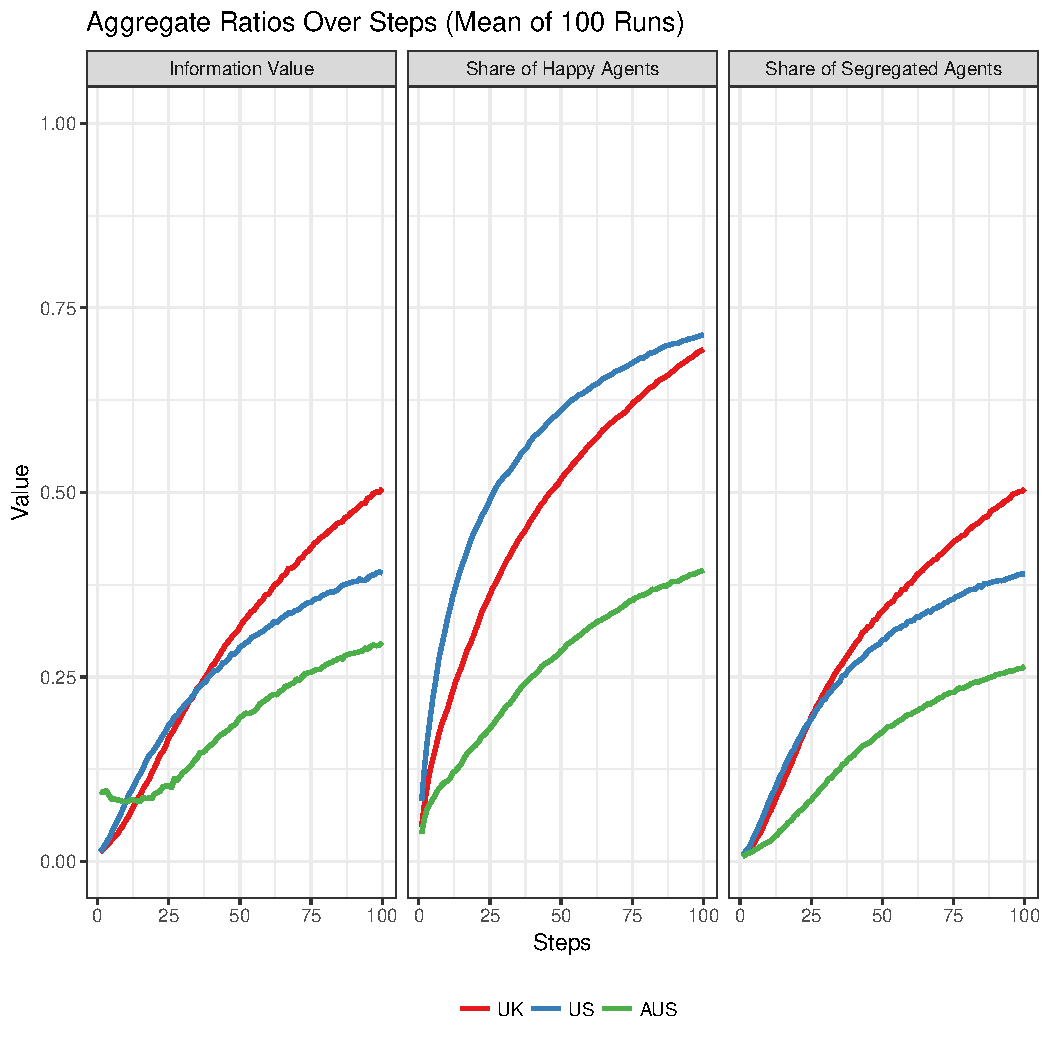
\includegraphics[height=10cm,width=16cm]{all_agg_ratios.pdf}
\end{figure}

\begin{figure}[bp!]
\centering
\caption{all grp ratios}
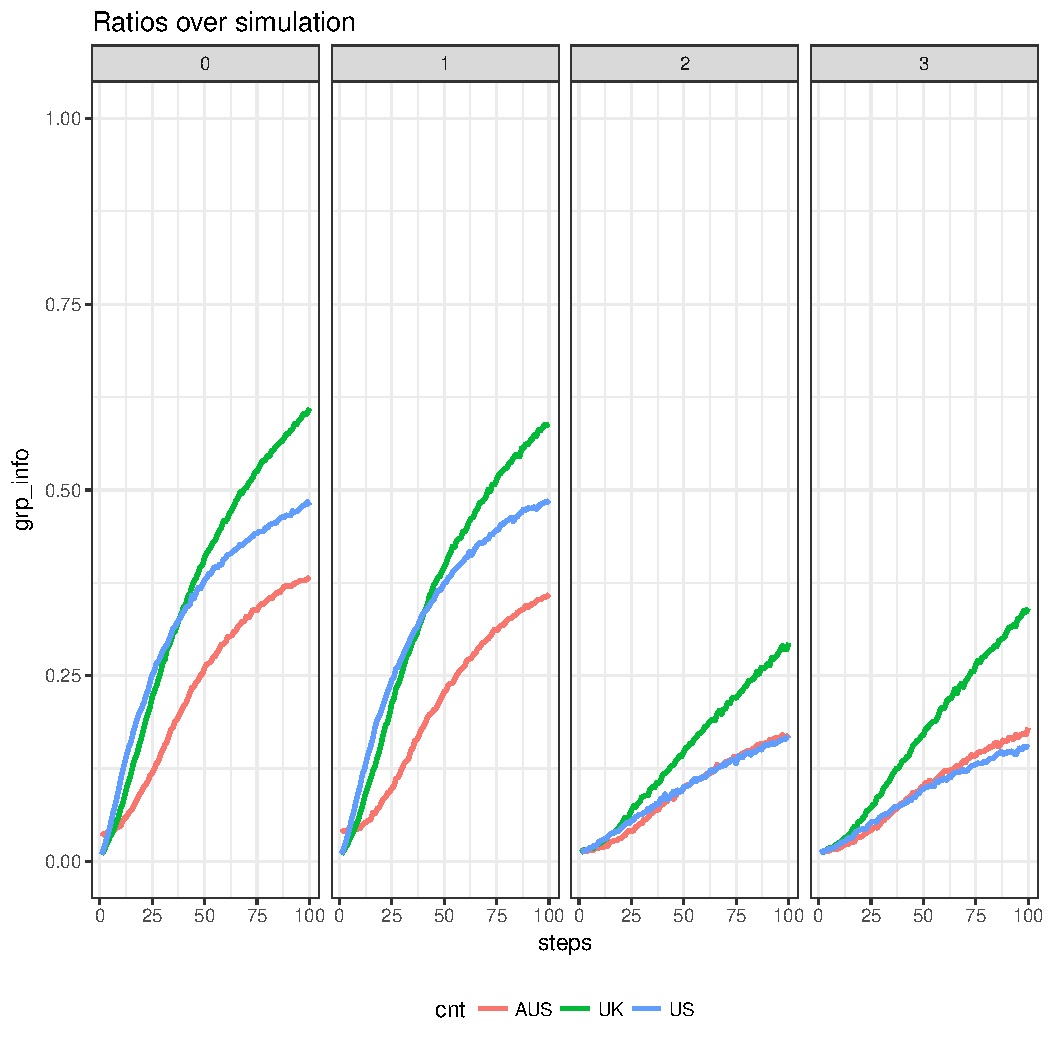
\includegraphics[height=10cm,width=16cm]{all_grp_ratios.pdf}
\end{figure}

\begin{table}[ht]
\centering
\caption{table}
\begin{tabular}{llll}
  \hline
Steps & Country & Happy & Segregated \\ 
  \hline \hline
25 & AUS & 16.99\% & 7.93\% \\ 
  25 & UK & 35.28\% & 18.48\% \\ 
  25 & US & 48.95\% & 19.81\% \\ \hline
  50 & AUS & 26.98\% & 16.82\% \\ 
  50 & UK & 51.70\% & 33.51\% \\ 
  50 & US & 61.12\% & 30.99\% \\  \hline
  75 & AUS & 34.00\% & 22.03\% \\ 
  75 & UK & 62.66\% & 43.51\% \\ 
  75 & US & 68.16\% & 37.00\% \\  \hline
  100 & AUS & 37.14\% & 24.99\% \\ 
  100 & UK & 70.14\% & 50.69\% \\ 
  100 & US & 71.93\% & 40.47\% \\ 
   \hline
\end{tabular}
\end{table}



%*******************************************************************************************************************************************************************
%*******************************************************************************************************************************************************************

\section{\label{sec_conc}Conclusion}


%*******************************************************************************************************************************************************************
%*******************************************************************************************************************************************************************

%reference section with econometrica style. there are two options. the first is to use a bibtex-file. this can be very helpful in a paper with many reference. the second is to write down the referenes by hand. 

\newpage

%Version 1
%\bibliographystyle{econometrica}
%\bibliography{bibliography}

%Version 2
\section*{\label{sec_ref}References}

BUSCH ET AL. (2014):`` Places and Preferences: A Longitudinal Analysis of Self-Selection and Contextual Effects,'' \textit{British Journal of Political Science} 46, 529-550.

\noindent MCDONALD, I. (2011):`` Migration and Sorting in the American Electorate: Evidence From the 2006 Cooperative Congressional Election Study,'' \textit{American Politics Research} 39(3), 512-533.

\noindent TAM CHO, W. K., GIMPEL, J. G. AND HUI, I. S (2012): ``Voter Migration and the Geographic Sorting of the
American Electorate,'' \textit{Annals of the Association of American Geographers}, DOI:10.1080/00045608.2012.720229.
 

\noindent ANGRIST, J. D., AND J. PISCHKE (2009): \textit{Mostly Harmless Econometrics: An Empiricist's Companion}. Princeton University Press.
    
\noindent KENNEDY, P. (2005): ``Oh No! I Got the Wrong Sign! What Should I Do?,'' \textit{Journal of Economic Education}, 36, 77--92.
    
\noindent LEAMER, E. E. (1975): ```Explaining Your Results' as Access-Biased Memory,'' \textit{Journal of the American Statistical Association}, 70, 88--93.
    
\noindent LEAMER, E. E. (1983): ``Let's Take the Con Out of Econometrics,'' \textit{American Economic Review}, 73, 31--43.
    
\noindent SALA-I-MARTIN, X. X. (1997): ``I Just Ran Two Million Regressions,'' \textit{American Economic Review}, 87, 178--183.

\noindent WOOLDRIDGE, J. M. (2008): \textit{Introductory Econometrics: A Modern Approach}. South-Western Cengage Learning.

%*******************************************************************************************************************************************************************
%*******************************************************************************************************************************************************************



\end{document}
%the  end 